%\renewcommand{\theequation}{\theenumi}
%\begin{enumerate}[label=\arabic*.,ref=\thesubsection.\theenumi]
%\numberwithin{equation}{enumi}
    \item Solve $30x < 200$ when
    \begin{enumerate} 
    \item  x is a natural number,
    \item x is an integer.
\end{enumerate}
\solution From the given information, 
\begin{align}
30x < 200 \implies x < \frac{20}{3}
\label{eq:lineq_nat}
\end{align}
If $x$ is a natural number, $x \in \cbrak{1, 2, 3, 4, 5, 6}$. If $x$ is an integer, then the solution set includes 0 as well as all negative integers.
    \item Solve $5x-3 < 3x+1$ when
    \begin{enumerate} 
\item  x is an integer,
    \item x is a real number.
\end{enumerate}
\solution 
\begin{align}
5x-3 < 3x+1 \implies x < 2
\label{eq:lineq_real}
\end{align}
%
If $x$ is real, then $x \in \brak{-\infty, 2}$. 
%Fig.  provides a graphical solution using the following python code
%\begin{lstlisting}
%\end{lstlisting}
    \item Solve the following system of linear inequalities graphically.
\begin{align}
\label{eq:line_two_ineq}
\begin{split}
    x+y &\geq 5
\\
    x-y &\leq 3
\end{split}
\end{align}
\solution  Let $u_1 \ge 0, u_2 \ge 0$.  This may be expressed as
\begin{align}
\vec{u} = \myvec{u_1\\u_2}\succeq \vec{0}
\end{align}
%
\eqref{eq:line_two_ineq} can then be expressed as
\begin{align}
\begin{split}
    x+y &\geq 5
\\
    -x+y &\geq -3
\end{split}
%
\\
\implies 
\myvec{1 & 1 \\ -1 & 1}\vec{x}  &\succeq \myvec{5\\-3}
\\
\myvec{1 & 1 \\ -1 & 1}\vec{x}  -\vec{u}&=\myvec{5\\-3}
\\
\text{or, }
\myvec{1 & 1 \\ -1 & 1}\vec{x} &= \myvec{5\\-3} +\vec{u}
\end{align}
%
resulting in 
\begin{align}
\vec{x} &= \myvec{1 & 1 \\ -1 & 1}^{-1}\myvec{5\\-3} +\myvec{1 & 1 \\ -1 & 1}^{-1}\vec{u}
\\
\text{or, } \vec{x} &= \myvec{4\\1} +\frac{1}{2}\myvec{1 & -1 \\ 1 & 1}\vec{u}
\end{align}
%
after obtaining the  inverse.
%
 Fig. \ref{fig:line_ineq} generated using the following python code shows the region satisfying \eqref{eq:line_two_ineq}

\begin{lstlisting}
codes/line/line_ineq.py
\end{lstlisting}
%
\begin{figure}[!ht]
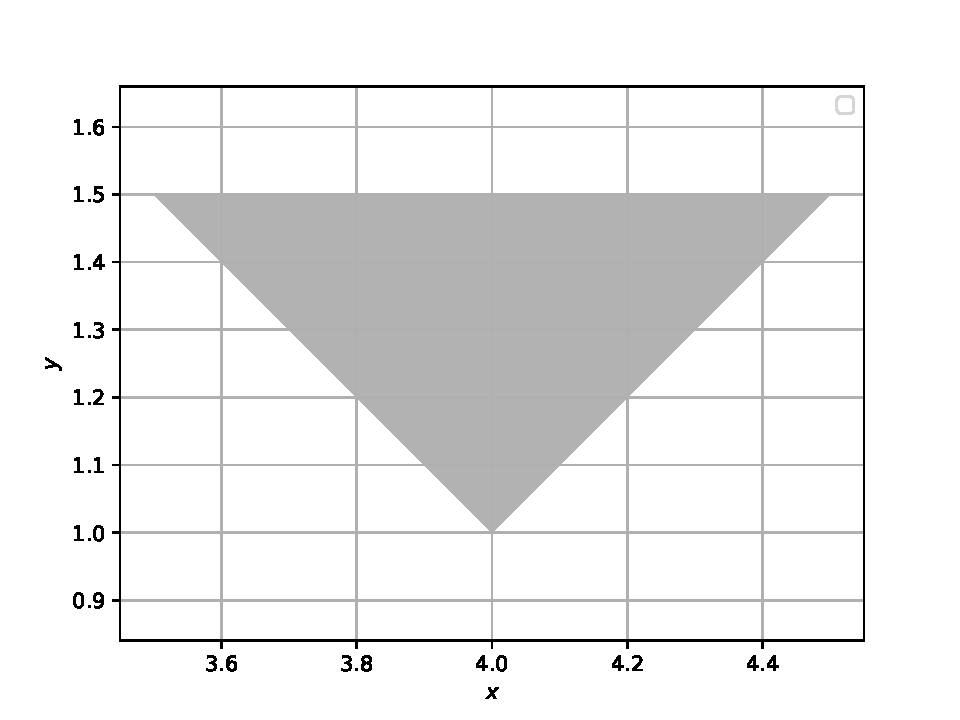
\includegraphics[width=\columnwidth]{./line/figs/line_ineq.eps}
\caption{}
\label{fig:line_ineq}
\end{figure}
%
\item Solve 
\begin{align}
\begin{split}
2x+y \geq 4
\\ 
x+y \leq 3
\\ 
2x-3y \leq 6
\end{split}
\label{eq:line_mult_ineq}
\end{align}
%
\\
\solution  Fig. \ref{fig:line_ineq_mult} generated using the following python code shows the region satisfying \eqref{eq:line_mult_ineq}

\begin{lstlisting}
codes/line/line_ineq_mult.py
\end{lstlisting}
%
\begin{figure}[!ht]
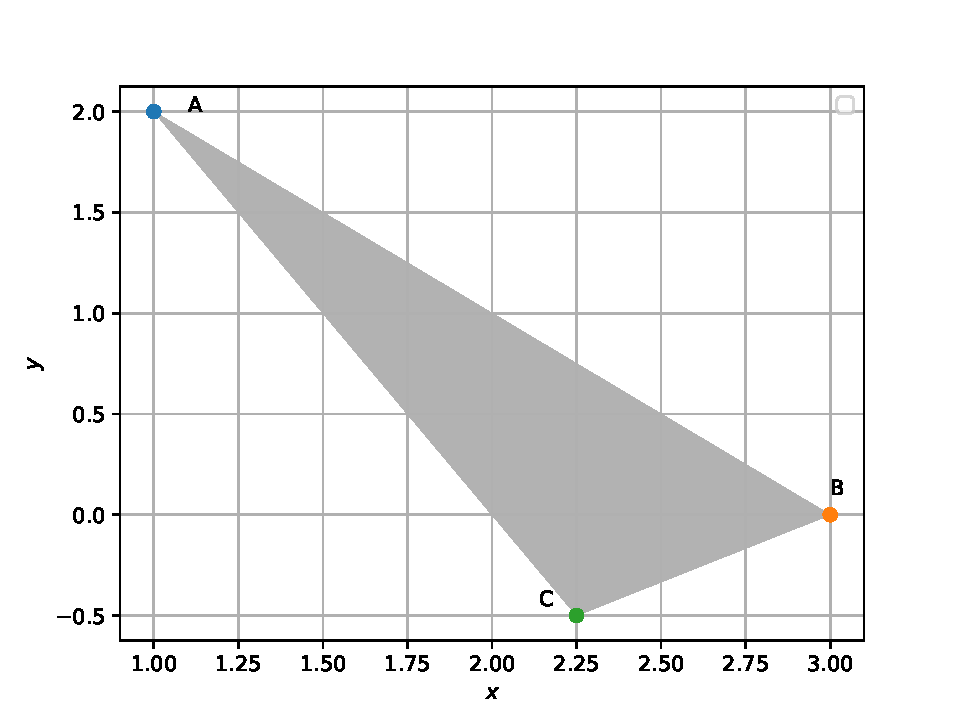
\includegraphics[width=\columnwidth]{./line/figs/line_ineq_mult.eps}
\caption{}
\label{fig:line_ineq_mult}
\end{figure}
%
\item   Solve    $x+y < 5$ graphically.
\\
\solution 
The following python code generates Fig. \ref{fig:3.11.5_qsix}.
	\begin{lstlisting}
	./solutions/5/codes/lines/q6.py
	\end{lstlisting}
	\begin{figure}[!ht]
	\centering
	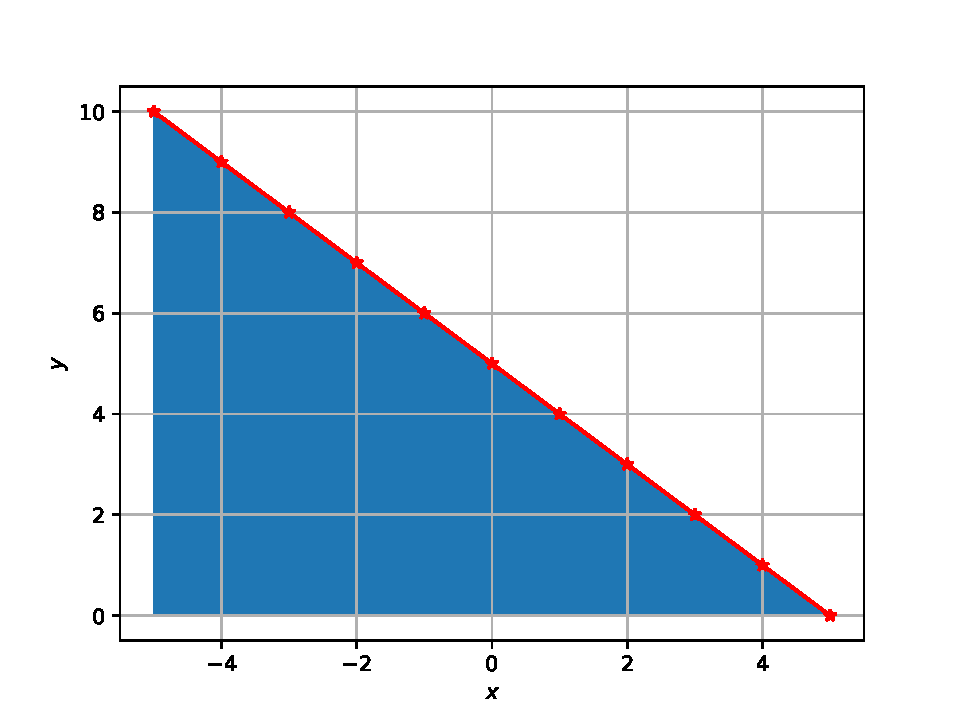
\includegraphics[width=\columnwidth]{./solutions/5/figs/lines/q6.eps}
	\caption{x+y$<$5}
	\label{fig:3.11.5_qsix}	
	\end{figure}
	

%
    \item Solve 
\begin{align}
\myvec{3 & 2 \\ 1 & 4 \\ 1 & 0 \\ 0 & -1 \\ -1 & 0} \vec{x}\preceq \myvec{150\\80\\15\\0\\0}
%3x+2y \leq 150
%\\ 
%x+4y \leq 80
%\\ 
%x \leq 15
%\\ 
%y \geq 0
%\\
%x \geq 0 
\end{align}
%
   
%    \end{enumerate}
\item Solve  x $\geq$ 3, y $\geq$ 2 graphically.
\\
\solution 
From theory, we understand that using dot product we can find the angle between the lines 
\begin{enumerate}
	\item 
	\begin{align}\label{eq:solutions/line_plane/74/codes:5}
		\frac{x-2}{2} = \frac{y-1}{5} &= \frac{z+3}{-3}, 
	\end{align}
	\begin{align}\label{eq:solutions/line_plane/74/codes:6}
		\frac{x+2}{-1} = \frac{y-4}{8} &= \frac{z-5}{4} 
	\end{align}


The above symmetric equations \ref{eq:solutions/line_plane/74/codes:5}, \ref{eq:solutions/line_plane/74/codes:6} can be represented in the vector form as 
\begin{align}\label{eq:solutions/line_plane/74/codes7}
	\quad \vec{r_1} &= \myvec{2\\1\\-3} + \lambda_1\myvec{2\\5\\-3}
	\\
	\quad \vec{r_2} &= \myvec{-2\\4\\5} + \lambda_2\myvec{-1\\8\\4}
\end{align}

As we have to find the angle between the vectors, we will only be taking the direction vectors into consideration. The direction vectors are $\vec{u}$ = $\myvec{2\\5\\-3}$ and $\vec{v}$ = $\myvec{-1\\8\\4}$. We can find the corresponding magnitude values

\begin{align}\label{eq:solutions/line_plane/74/codes9}
	\norm{\vec{u}} =\sqrt{2^{2}+5^{2}+(-3)^{2}} =\sqrt{38}
\end{align}
\begin{align}\label{eq:solutions/line_plane/74/codes10}
	\norm{\vec{v}} =\sqrt{(-1)^{2}+8^{2}+4^{2}} =\sqrt{81}
\end{align}

Using \ref{eq:solutions/line_plane/74/codes4}, \ref{eq:solutions/line_plane/74/codes9}, \ref{eq:solutions/line_plane/74/codes10} we get
\begin{align}
	\theta = \cos ^{-1}\frac{\myvec{2\\5\\-3}^{T}\myvec{-1\\8\\4}}{(\sqrt{38})(\sqrt{81})} 
	\\
	\theta = \cos ^{-1}\frac{26}{55.4797}
	\\
	\theta = \cos ^{-1} (0.4686)
	\\
	\theta = 62.053\degree
\end{align}

Therefore, the angle between the two lines is $62.053\degree$.See Fig. \ref{fig:solutions/line_plane/74/codesline_equation_1}

\begin{figure}
	\centering
	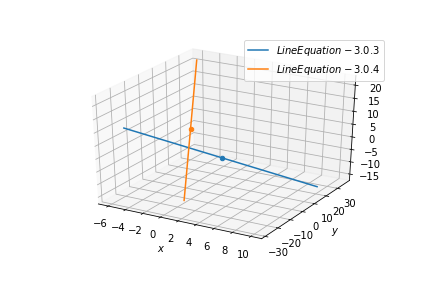
\includegraphics[width=\columnwidth]{./solutions/line_plane/74/codes/figs/Line_interest_1.png}
	\caption{Graph for equations \ref{eq:solutions/line_plane/74/codes7}}
	\label{fig:solutions/line_plane/74/codesline_equation_1}
\end{figure}


	\item 
	\begin{align}\label{eq:solutions/line_plane/74/codes12}
		\frac{x}{2} = \frac{y}{2} &= \frac{z}{1}, 
	\end{align}
	\begin{align}\label{eq:solutions/line_plane/74/codes13}
		\frac{x-5}{4} = \frac{y-2}{1} &= \frac{z-3}{8} 
	\end{align}



The above symmetric equations \ref{eq:solutions/line_plane/74/codes12}, \ref{eq:solutions/line_plane/74/codes13} can be represented in the vector form as 
\begin{align}\label{eq:solutions/line_plane/74/codes14}
	\quad \vec{r_1} &= \myvec{0\\0\\0} + \lambda_1\myvec{2\\2\\1}
	\\
	\quad \vec{r_2} &= \myvec{5\\2\\3} + \lambda_2\myvec{4\\1\\8}
\end{align}

As we have to find the angle between the vectors, we will only be taking the direction vectors into consideration. The direction vectors are $\vec{u}$ = $\myvec{2\\2\\1}$ and $\vec{v}$ = $\myvec{4\\1\\8}$. We can find the corresponding magnitude values

\begin{align}\label{eq:solutions/line_plane/74/codes16}
	\norm{\vec{u}} =\sqrt{2^{2}+2^{2}+1^{2}} =\sqrt{9}
\end{align}
\begin{align}\label{eq:solutions/line_plane/74/codes17}
	\norm{\vec{v}} =\sqrt{4^{2}+1^{2}+8^{2}} =\sqrt{81}
\end{align}

Using \ref{eq:solutions/line_plane/74/codes4}, \ref{eq:solutions/line_plane/74/codes16}, \ref{eq:solutions/line_plane/74/codes17} we get
\begin{align}
	\theta = \cos ^{-1}\frac{\myvec{2\\2\\1}^{T}\myvec{4\\1\\8}}{(\sqrt{9})(\sqrt{81})} 
	\\
	\theta = \cos ^{-1}\frac{18}{27.00}
	\\
	\theta = \cos ^{-1} (0.667)
	\\
	\theta = 48.189\degree
\end{align}

Therefore, the angle between the two lines is $48.189\degree$. See Fig. \ref{fig:solutions/line_plane/74/codesline_equation_2}


\begin{figure}
	\centering
	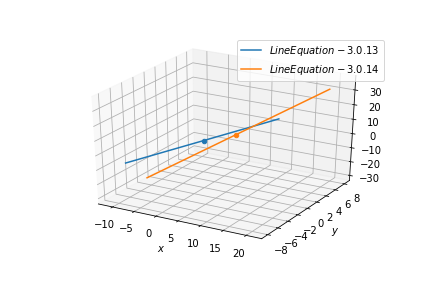
\includegraphics[width=\columnwidth]{./solutions/line_plane/74/codes/figs/Line_interest_2.png}
	\caption{Graph for equations \ref{eq:solutions/line_plane/74/codes14}}
	\label{fig:solutions/line_plane/74/codesline_equation_2}
\end{figure}
\end{enumerate}

    


    \item Solve 7x+3 $<$ 5x+9. Show the graph of the solutions on number line.
\\
\solution 
From theory, we understand that using dot product we can find the angle between the lines 
\begin{enumerate}
	\item 
	\begin{align}\label{eq:solutions/line_plane/74/codes:5}
		\frac{x-2}{2} = \frac{y-1}{5} &= \frac{z+3}{-3}, 
	\end{align}
	\begin{align}\label{eq:solutions/line_plane/74/codes:6}
		\frac{x+2}{-1} = \frac{y-4}{8} &= \frac{z-5}{4} 
	\end{align}


The above symmetric equations \ref{eq:solutions/line_plane/74/codes:5}, \ref{eq:solutions/line_plane/74/codes:6} can be represented in the vector form as 
\begin{align}\label{eq:solutions/line_plane/74/codes7}
	\quad \vec{r_1} &= \myvec{2\\1\\-3} + \lambda_1\myvec{2\\5\\-3}
	\\
	\quad \vec{r_2} &= \myvec{-2\\4\\5} + \lambda_2\myvec{-1\\8\\4}
\end{align}

As we have to find the angle between the vectors, we will only be taking the direction vectors into consideration. The direction vectors are $\vec{u}$ = $\myvec{2\\5\\-3}$ and $\vec{v}$ = $\myvec{-1\\8\\4}$. We can find the corresponding magnitude values

\begin{align}\label{eq:solutions/line_plane/74/codes9}
	\norm{\vec{u}} =\sqrt{2^{2}+5^{2}+(-3)^{2}} =\sqrt{38}
\end{align}
\begin{align}\label{eq:solutions/line_plane/74/codes10}
	\norm{\vec{v}} =\sqrt{(-1)^{2}+8^{2}+4^{2}} =\sqrt{81}
\end{align}

Using \ref{eq:solutions/line_plane/74/codes4}, \ref{eq:solutions/line_plane/74/codes9}, \ref{eq:solutions/line_plane/74/codes10} we get
\begin{align}
	\theta = \cos ^{-1}\frac{\myvec{2\\5\\-3}^{T}\myvec{-1\\8\\4}}{(\sqrt{38})(\sqrt{81})} 
	\\
	\theta = \cos ^{-1}\frac{26}{55.4797}
	\\
	\theta = \cos ^{-1} (0.4686)
	\\
	\theta = 62.053\degree
\end{align}

Therefore, the angle between the two lines is $62.053\degree$.See Fig. \ref{fig:solutions/line_plane/74/codesline_equation_1}

\begin{figure}
	\centering
	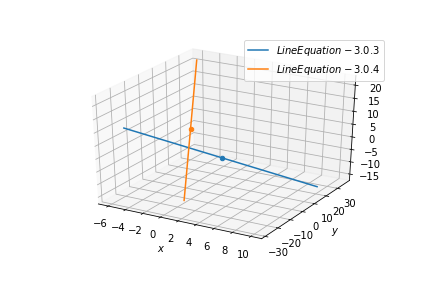
\includegraphics[width=\columnwidth]{./solutions/line_plane/74/codes/figs/Line_interest_1.png}
	\caption{Graph for equations \ref{eq:solutions/line_plane/74/codes7}}
	\label{fig:solutions/line_plane/74/codesline_equation_1}
\end{figure}


	\item 
	\begin{align}\label{eq:solutions/line_plane/74/codes12}
		\frac{x}{2} = \frac{y}{2} &= \frac{z}{1}, 
	\end{align}
	\begin{align}\label{eq:solutions/line_plane/74/codes13}
		\frac{x-5}{4} = \frac{y-2}{1} &= \frac{z-3}{8} 
	\end{align}



The above symmetric equations \ref{eq:solutions/line_plane/74/codes12}, \ref{eq:solutions/line_plane/74/codes13} can be represented in the vector form as 
\begin{align}\label{eq:solutions/line_plane/74/codes14}
	\quad \vec{r_1} &= \myvec{0\\0\\0} + \lambda_1\myvec{2\\2\\1}
	\\
	\quad \vec{r_2} &= \myvec{5\\2\\3} + \lambda_2\myvec{4\\1\\8}
\end{align}

As we have to find the angle between the vectors, we will only be taking the direction vectors into consideration. The direction vectors are $\vec{u}$ = $\myvec{2\\2\\1}$ and $\vec{v}$ = $\myvec{4\\1\\8}$. We can find the corresponding magnitude values

\begin{align}\label{eq:solutions/line_plane/74/codes16}
	\norm{\vec{u}} =\sqrt{2^{2}+2^{2}+1^{2}} =\sqrt{9}
\end{align}
\begin{align}\label{eq:solutions/line_plane/74/codes17}
	\norm{\vec{v}} =\sqrt{4^{2}+1^{2}+8^{2}} =\sqrt{81}
\end{align}

Using \ref{eq:solutions/line_plane/74/codes4}, \ref{eq:solutions/line_plane/74/codes16}, \ref{eq:solutions/line_plane/74/codes17} we get
\begin{align}
	\theta = \cos ^{-1}\frac{\myvec{2\\2\\1}^{T}\myvec{4\\1\\8}}{(\sqrt{9})(\sqrt{81})} 
	\\
	\theta = \cos ^{-1}\frac{18}{27.00}
	\\
	\theta = \cos ^{-1} (0.667)
	\\
	\theta = 48.189\degree
\end{align}

Therefore, the angle between the two lines is $48.189\degree$. See Fig. \ref{fig:solutions/line_plane/74/codesline_equation_2}


\begin{figure}
	\centering
	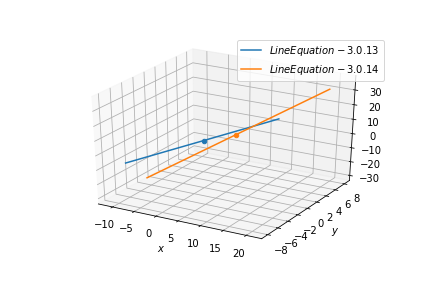
\includegraphics[width=\columnwidth]{./solutions/line_plane/74/codes/figs/Line_interest_2.png}
	\caption{Graph for equations \ref{eq:solutions/line_plane/74/codes14}}
	\label{fig:solutions/line_plane/74/codesline_equation_2}
\end{figure}
\end{enumerate}

    

    \item Solve $\frac{3x-4}{2} \geq \frac{x+1}{4}-1$. Show the graph of the solutions on number line.
\\
\solution 
From theory, we understand that using dot product we can find the angle between the lines 
\begin{enumerate}
	\item 
	\begin{align}\label{eq:solutions/line_plane/74/codes:5}
		\frac{x-2}{2} = \frac{y-1}{5} &= \frac{z+3}{-3}, 
	\end{align}
	\begin{align}\label{eq:solutions/line_plane/74/codes:6}
		\frac{x+2}{-1} = \frac{y-4}{8} &= \frac{z-5}{4} 
	\end{align}


The above symmetric equations \ref{eq:solutions/line_plane/74/codes:5}, \ref{eq:solutions/line_plane/74/codes:6} can be represented in the vector form as 
\begin{align}\label{eq:solutions/line_plane/74/codes7}
	\quad \vec{r_1} &= \myvec{2\\1\\-3} + \lambda_1\myvec{2\\5\\-3}
	\\
	\quad \vec{r_2} &= \myvec{-2\\4\\5} + \lambda_2\myvec{-1\\8\\4}
\end{align}

As we have to find the angle between the vectors, we will only be taking the direction vectors into consideration. The direction vectors are $\vec{u}$ = $\myvec{2\\5\\-3}$ and $\vec{v}$ = $\myvec{-1\\8\\4}$. We can find the corresponding magnitude values

\begin{align}\label{eq:solutions/line_plane/74/codes9}
	\norm{\vec{u}} =\sqrt{2^{2}+5^{2}+(-3)^{2}} =\sqrt{38}
\end{align}
\begin{align}\label{eq:solutions/line_plane/74/codes10}
	\norm{\vec{v}} =\sqrt{(-1)^{2}+8^{2}+4^{2}} =\sqrt{81}
\end{align}

Using \ref{eq:solutions/line_plane/74/codes4}, \ref{eq:solutions/line_plane/74/codes9}, \ref{eq:solutions/line_plane/74/codes10} we get
\begin{align}
	\theta = \cos ^{-1}\frac{\myvec{2\\5\\-3}^{T}\myvec{-1\\8\\4}}{(\sqrt{38})(\sqrt{81})} 
	\\
	\theta = \cos ^{-1}\frac{26}{55.4797}
	\\
	\theta = \cos ^{-1} (0.4686)
	\\
	\theta = 62.053\degree
\end{align}

Therefore, the angle between the two lines is $62.053\degree$.See Fig. \ref{fig:solutions/line_plane/74/codesline_equation_1}

\begin{figure}
	\centering
	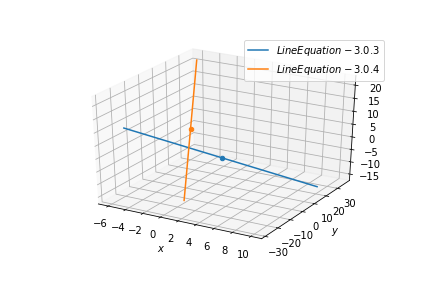
\includegraphics[width=\columnwidth]{./solutions/line_plane/74/codes/figs/Line_interest_1.png}
	\caption{Graph for equations \ref{eq:solutions/line_plane/74/codes7}}
	\label{fig:solutions/line_plane/74/codesline_equation_1}
\end{figure}


	\item 
	\begin{align}\label{eq:solutions/line_plane/74/codes12}
		\frac{x}{2} = \frac{y}{2} &= \frac{z}{1}, 
	\end{align}
	\begin{align}\label{eq:solutions/line_plane/74/codes13}
		\frac{x-5}{4} = \frac{y-2}{1} &= \frac{z-3}{8} 
	\end{align}



The above symmetric equations \ref{eq:solutions/line_plane/74/codes12}, \ref{eq:solutions/line_plane/74/codes13} can be represented in the vector form as 
\begin{align}\label{eq:solutions/line_plane/74/codes14}
	\quad \vec{r_1} &= \myvec{0\\0\\0} + \lambda_1\myvec{2\\2\\1}
	\\
	\quad \vec{r_2} &= \myvec{5\\2\\3} + \lambda_2\myvec{4\\1\\8}
\end{align}

As we have to find the angle between the vectors, we will only be taking the direction vectors into consideration. The direction vectors are $\vec{u}$ = $\myvec{2\\2\\1}$ and $\vec{v}$ = $\myvec{4\\1\\8}$. We can find the corresponding magnitude values

\begin{align}\label{eq:solutions/line_plane/74/codes16}
	\norm{\vec{u}} =\sqrt{2^{2}+2^{2}+1^{2}} =\sqrt{9}
\end{align}
\begin{align}\label{eq:solutions/line_plane/74/codes17}
	\norm{\vec{v}} =\sqrt{4^{2}+1^{2}+8^{2}} =\sqrt{81}
\end{align}

Using \ref{eq:solutions/line_plane/74/codes4}, \ref{eq:solutions/line_plane/74/codes16}, \ref{eq:solutions/line_plane/74/codes17} we get
\begin{align}
	\theta = \cos ^{-1}\frac{\myvec{2\\2\\1}^{T}\myvec{4\\1\\8}}{(\sqrt{9})(\sqrt{81})} 
	\\
	\theta = \cos ^{-1}\frac{18}{27.00}
	\\
	\theta = \cos ^{-1} (0.667)
	\\
	\theta = 48.189\degree
\end{align}

Therefore, the angle between the two lines is $48.189\degree$. See Fig. \ref{fig:solutions/line_plane/74/codesline_equation_2}


\begin{figure}
	\centering
	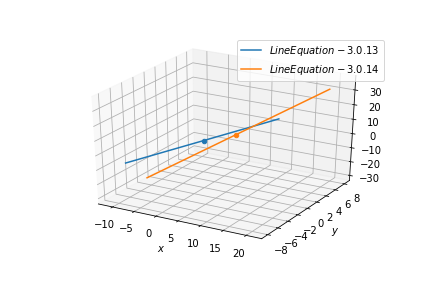
\includegraphics[width=\columnwidth]{./solutions/line_plane/74/codes/figs/Line_interest_2.png}
	\caption{Graph for equations \ref{eq:solutions/line_plane/74/codes14}}
	\label{fig:solutions/line_plane/74/codesline_equation_2}
\end{figure}
\end{enumerate}

    

    \item The marks obtained by a student of Class XI in first and second terminal examination are 62 and 48, respectively. Find the minimum marks he should get in the annual examination to have an average of at least 60 marks.
\\
\solution 
From theory, we understand that using dot product we can find the angle between the lines 
\begin{enumerate}
	\item 
	\begin{align}\label{eq:solutions/line_plane/74/codes:5}
		\frac{x-2}{2} = \frac{y-1}{5} &= \frac{z+3}{-3}, 
	\end{align}
	\begin{align}\label{eq:solutions/line_plane/74/codes:6}
		\frac{x+2}{-1} = \frac{y-4}{8} &= \frac{z-5}{4} 
	\end{align}


The above symmetric equations \ref{eq:solutions/line_plane/74/codes:5}, \ref{eq:solutions/line_plane/74/codes:6} can be represented in the vector form as 
\begin{align}\label{eq:solutions/line_plane/74/codes7}
	\quad \vec{r_1} &= \myvec{2\\1\\-3} + \lambda_1\myvec{2\\5\\-3}
	\\
	\quad \vec{r_2} &= \myvec{-2\\4\\5} + \lambda_2\myvec{-1\\8\\4}
\end{align}

As we have to find the angle between the vectors, we will only be taking the direction vectors into consideration. The direction vectors are $\vec{u}$ = $\myvec{2\\5\\-3}$ and $\vec{v}$ = $\myvec{-1\\8\\4}$. We can find the corresponding magnitude values

\begin{align}\label{eq:solutions/line_plane/74/codes9}
	\norm{\vec{u}} =\sqrt{2^{2}+5^{2}+(-3)^{2}} =\sqrt{38}
\end{align}
\begin{align}\label{eq:solutions/line_plane/74/codes10}
	\norm{\vec{v}} =\sqrt{(-1)^{2}+8^{2}+4^{2}} =\sqrt{81}
\end{align}

Using \ref{eq:solutions/line_plane/74/codes4}, \ref{eq:solutions/line_plane/74/codes9}, \ref{eq:solutions/line_plane/74/codes10} we get
\begin{align}
	\theta = \cos ^{-1}\frac{\myvec{2\\5\\-3}^{T}\myvec{-1\\8\\4}}{(\sqrt{38})(\sqrt{81})} 
	\\
	\theta = \cos ^{-1}\frac{26}{55.4797}
	\\
	\theta = \cos ^{-1} (0.4686)
	\\
	\theta = 62.053\degree
\end{align}

Therefore, the angle between the two lines is $62.053\degree$.See Fig. \ref{fig:solutions/line_plane/74/codesline_equation_1}

\begin{figure}
	\centering
	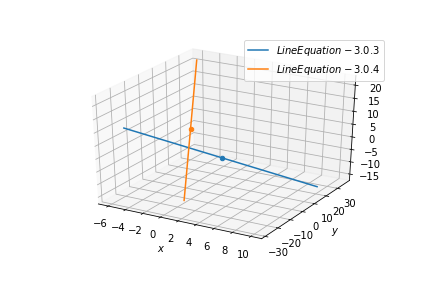
\includegraphics[width=\columnwidth]{./solutions/line_plane/74/codes/figs/Line_interest_1.png}
	\caption{Graph for equations \ref{eq:solutions/line_plane/74/codes7}}
	\label{fig:solutions/line_plane/74/codesline_equation_1}
\end{figure}


	\item 
	\begin{align}\label{eq:solutions/line_plane/74/codes12}
		\frac{x}{2} = \frac{y}{2} &= \frac{z}{1}, 
	\end{align}
	\begin{align}\label{eq:solutions/line_plane/74/codes13}
		\frac{x-5}{4} = \frac{y-2}{1} &= \frac{z-3}{8} 
	\end{align}



The above symmetric equations \ref{eq:solutions/line_plane/74/codes12}, \ref{eq:solutions/line_plane/74/codes13} can be represented in the vector form as 
\begin{align}\label{eq:solutions/line_plane/74/codes14}
	\quad \vec{r_1} &= \myvec{0\\0\\0} + \lambda_1\myvec{2\\2\\1}
	\\
	\quad \vec{r_2} &= \myvec{5\\2\\3} + \lambda_2\myvec{4\\1\\8}
\end{align}

As we have to find the angle between the vectors, we will only be taking the direction vectors into consideration. The direction vectors are $\vec{u}$ = $\myvec{2\\2\\1}$ and $\vec{v}$ = $\myvec{4\\1\\8}$. We can find the corresponding magnitude values

\begin{align}\label{eq:solutions/line_plane/74/codes16}
	\norm{\vec{u}} =\sqrt{2^{2}+2^{2}+1^{2}} =\sqrt{9}
\end{align}
\begin{align}\label{eq:solutions/line_plane/74/codes17}
	\norm{\vec{v}} =\sqrt{4^{2}+1^{2}+8^{2}} =\sqrt{81}
\end{align}

Using \ref{eq:solutions/line_plane/74/codes4}, \ref{eq:solutions/line_plane/74/codes16}, \ref{eq:solutions/line_plane/74/codes17} we get
\begin{align}
	\theta = \cos ^{-1}\frac{\myvec{2\\2\\1}^{T}\myvec{4\\1\\8}}{(\sqrt{9})(\sqrt{81})} 
	\\
	\theta = \cos ^{-1}\frac{18}{27.00}
	\\
	\theta = \cos ^{-1} (0.667)
	\\
	\theta = 48.189\degree
\end{align}

Therefore, the angle between the two lines is $48.189\degree$. See Fig. \ref{fig:solutions/line_plane/74/codesline_equation_2}


\begin{figure}
	\centering
	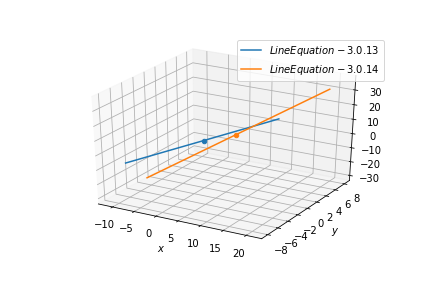
\includegraphics[width=\columnwidth]{./solutions/line_plane/74/codes/figs/Line_interest_2.png}
	\caption{Graph for equations \ref{eq:solutions/line_plane/74/codes14}}
	\label{fig:solutions/line_plane/74/codesline_equation_2}
\end{figure}
\end{enumerate}

    

    \item Find all pairs of consecutive odd natural numbers, both of which are larger than 10, such that their sum is less than 40.
\\
\solution 
	
Let x be an odd natural number and y be the odd natural number consecutive to x.
	\begin{align}
	\therefore y=x+2
	\end{align}
	We need to find x and y  such that 
	\begin{multline}
x,y >10 \text{ and } x+y<40\\
\therefore x+x+2<40\\
2x+2<40\\
x+1<20\\
x<19
	\end{multline}
	
	
	Hence the condition is satisfied when $x>10$ and $x<19$
	
	
	
	The following python code computes the required pairs of consecutive odd natural numbers which satisfy the required condition, shown in Fig.\ref{fig:3.11.5_fifteen}.
	\begin{lstlisting}
	./solutions/5/codes/lines/q15.py
	\end{lstlisting}
	\begin{figure}[!ht]
	\centering
	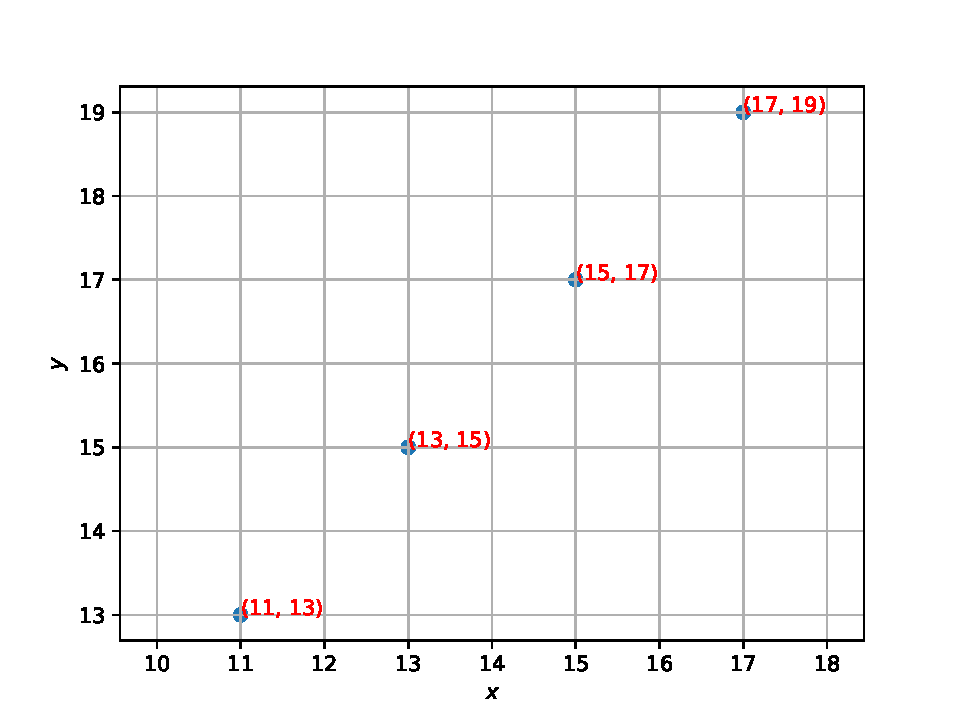
\includegraphics[width=\columnwidth]{./solutions/5/figs/lines/q15.eps}
	\caption{}
	\label{fig:3.11.5_fifteen}	
	\end{figure}

    \item Solve 3x+2y $>$ 6 graphically.
\\
\solution 
From theory, we understand that using dot product we can find the angle between the lines 
\begin{enumerate}
	\item 
	\begin{align}\label{eq:solutions/line_plane/74/codes:5}
		\frac{x-2}{2} = \frac{y-1}{5} &= \frac{z+3}{-3}, 
	\end{align}
	\begin{align}\label{eq:solutions/line_plane/74/codes:6}
		\frac{x+2}{-1} = \frac{y-4}{8} &= \frac{z-5}{4} 
	\end{align}


The above symmetric equations \ref{eq:solutions/line_plane/74/codes:5}, \ref{eq:solutions/line_plane/74/codes:6} can be represented in the vector form as 
\begin{align}\label{eq:solutions/line_plane/74/codes7}
	\quad \vec{r_1} &= \myvec{2\\1\\-3} + \lambda_1\myvec{2\\5\\-3}
	\\
	\quad \vec{r_2} &= \myvec{-2\\4\\5} + \lambda_2\myvec{-1\\8\\4}
\end{align}

As we have to find the angle between the vectors, we will only be taking the direction vectors into consideration. The direction vectors are $\vec{u}$ = $\myvec{2\\5\\-3}$ and $\vec{v}$ = $\myvec{-1\\8\\4}$. We can find the corresponding magnitude values

\begin{align}\label{eq:solutions/line_plane/74/codes9}
	\norm{\vec{u}} =\sqrt{2^{2}+5^{2}+(-3)^{2}} =\sqrt{38}
\end{align}
\begin{align}\label{eq:solutions/line_plane/74/codes10}
	\norm{\vec{v}} =\sqrt{(-1)^{2}+8^{2}+4^{2}} =\sqrt{81}
\end{align}

Using \ref{eq:solutions/line_plane/74/codes4}, \ref{eq:solutions/line_plane/74/codes9}, \ref{eq:solutions/line_plane/74/codes10} we get
\begin{align}
	\theta = \cos ^{-1}\frac{\myvec{2\\5\\-3}^{T}\myvec{-1\\8\\4}}{(\sqrt{38})(\sqrt{81})} 
	\\
	\theta = \cos ^{-1}\frac{26}{55.4797}
	\\
	\theta = \cos ^{-1} (0.4686)
	\\
	\theta = 62.053\degree
\end{align}

Therefore, the angle between the two lines is $62.053\degree$.See Fig. \ref{fig:solutions/line_plane/74/codesline_equation_1}

\begin{figure}
	\centering
	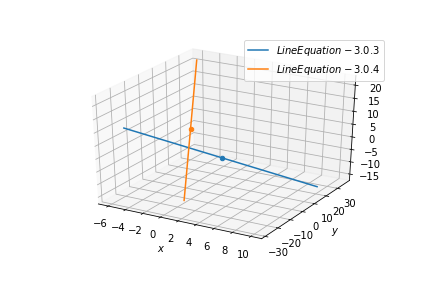
\includegraphics[width=\columnwidth]{./solutions/line_plane/74/codes/figs/Line_interest_1.png}
	\caption{Graph for equations \ref{eq:solutions/line_plane/74/codes7}}
	\label{fig:solutions/line_plane/74/codesline_equation_1}
\end{figure}


	\item 
	\begin{align}\label{eq:solutions/line_plane/74/codes12}
		\frac{x}{2} = \frac{y}{2} &= \frac{z}{1}, 
	\end{align}
	\begin{align}\label{eq:solutions/line_plane/74/codes13}
		\frac{x-5}{4} = \frac{y-2}{1} &= \frac{z-3}{8} 
	\end{align}



The above symmetric equations \ref{eq:solutions/line_plane/74/codes12}, \ref{eq:solutions/line_plane/74/codes13} can be represented in the vector form as 
\begin{align}\label{eq:solutions/line_plane/74/codes14}
	\quad \vec{r_1} &= \myvec{0\\0\\0} + \lambda_1\myvec{2\\2\\1}
	\\
	\quad \vec{r_2} &= \myvec{5\\2\\3} + \lambda_2\myvec{4\\1\\8}
\end{align}

As we have to find the angle between the vectors, we will only be taking the direction vectors into consideration. The direction vectors are $\vec{u}$ = $\myvec{2\\2\\1}$ and $\vec{v}$ = $\myvec{4\\1\\8}$. We can find the corresponding magnitude values

\begin{align}\label{eq:solutions/line_plane/74/codes16}
	\norm{\vec{u}} =\sqrt{2^{2}+2^{2}+1^{2}} =\sqrt{9}
\end{align}
\begin{align}\label{eq:solutions/line_plane/74/codes17}
	\norm{\vec{v}} =\sqrt{4^{2}+1^{2}+8^{2}} =\sqrt{81}
\end{align}

Using \ref{eq:solutions/line_plane/74/codes4}, \ref{eq:solutions/line_plane/74/codes16}, \ref{eq:solutions/line_plane/74/codes17} we get
\begin{align}
	\theta = \cos ^{-1}\frac{\myvec{2\\2\\1}^{T}\myvec{4\\1\\8}}{(\sqrt{9})(\sqrt{81})} 
	\\
	\theta = \cos ^{-1}\frac{18}{27.00}
	\\
	\theta = \cos ^{-1} (0.667)
	\\
	\theta = 48.189\degree
\end{align}

Therefore, the angle between the two lines is $48.189\degree$. See Fig. \ref{fig:solutions/line_plane/74/codesline_equation_2}


\begin{figure}
	\centering
	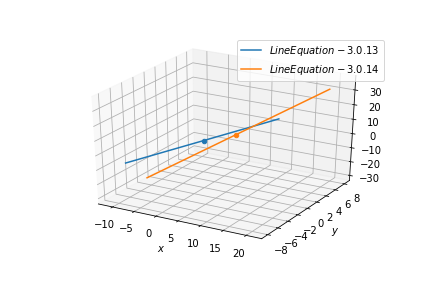
\includegraphics[width=\columnwidth]{./solutions/line_plane/74/codes/figs/Line_interest_2.png}
	\caption{Graph for equations \ref{eq:solutions/line_plane/74/codes14}}
	\label{fig:solutions/line_plane/74/codesline_equation_2}
\end{figure}
\end{enumerate}

    

    \item Solve 3x-6 $\geq$ 0 graphically in a two dimensional plane.
\\
\solution 
From theory, we understand that using dot product we can find the angle between the lines 
\begin{enumerate}
	\item 
	\begin{align}\label{eq:solutions/line_plane/74/codes:5}
		\frac{x-2}{2} = \frac{y-1}{5} &= \frac{z+3}{-3}, 
	\end{align}
	\begin{align}\label{eq:solutions/line_plane/74/codes:6}
		\frac{x+2}{-1} = \frac{y-4}{8} &= \frac{z-5}{4} 
	\end{align}


The above symmetric equations \ref{eq:solutions/line_plane/74/codes:5}, \ref{eq:solutions/line_plane/74/codes:6} can be represented in the vector form as 
\begin{align}\label{eq:solutions/line_plane/74/codes7}
	\quad \vec{r_1} &= \myvec{2\\1\\-3} + \lambda_1\myvec{2\\5\\-3}
	\\
	\quad \vec{r_2} &= \myvec{-2\\4\\5} + \lambda_2\myvec{-1\\8\\4}
\end{align}

As we have to find the angle between the vectors, we will only be taking the direction vectors into consideration. The direction vectors are $\vec{u}$ = $\myvec{2\\5\\-3}$ and $\vec{v}$ = $\myvec{-1\\8\\4}$. We can find the corresponding magnitude values

\begin{align}\label{eq:solutions/line_plane/74/codes9}
	\norm{\vec{u}} =\sqrt{2^{2}+5^{2}+(-3)^{2}} =\sqrt{38}
\end{align}
\begin{align}\label{eq:solutions/line_plane/74/codes10}
	\norm{\vec{v}} =\sqrt{(-1)^{2}+8^{2}+4^{2}} =\sqrt{81}
\end{align}

Using \ref{eq:solutions/line_plane/74/codes4}, \ref{eq:solutions/line_plane/74/codes9}, \ref{eq:solutions/line_plane/74/codes10} we get
\begin{align}
	\theta = \cos ^{-1}\frac{\myvec{2\\5\\-3}^{T}\myvec{-1\\8\\4}}{(\sqrt{38})(\sqrt{81})} 
	\\
	\theta = \cos ^{-1}\frac{26}{55.4797}
	\\
	\theta = \cos ^{-1} (0.4686)
	\\
	\theta = 62.053\degree
\end{align}

Therefore, the angle between the two lines is $62.053\degree$.See Fig. \ref{fig:solutions/line_plane/74/codesline_equation_1}

\begin{figure}
	\centering
	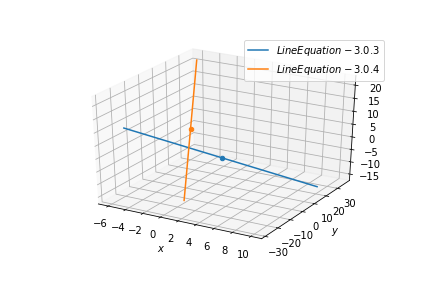
\includegraphics[width=\columnwidth]{./solutions/line_plane/74/codes/figs/Line_interest_1.png}
	\caption{Graph for equations \ref{eq:solutions/line_plane/74/codes7}}
	\label{fig:solutions/line_plane/74/codesline_equation_1}
\end{figure}


	\item 
	\begin{align}\label{eq:solutions/line_plane/74/codes12}
		\frac{x}{2} = \frac{y}{2} &= \frac{z}{1}, 
	\end{align}
	\begin{align}\label{eq:solutions/line_plane/74/codes13}
		\frac{x-5}{4} = \frac{y-2}{1} &= \frac{z-3}{8} 
	\end{align}



The above symmetric equations \ref{eq:solutions/line_plane/74/codes12}, \ref{eq:solutions/line_plane/74/codes13} can be represented in the vector form as 
\begin{align}\label{eq:solutions/line_plane/74/codes14}
	\quad \vec{r_1} &= \myvec{0\\0\\0} + \lambda_1\myvec{2\\2\\1}
	\\
	\quad \vec{r_2} &= \myvec{5\\2\\3} + \lambda_2\myvec{4\\1\\8}
\end{align}

As we have to find the angle between the vectors, we will only be taking the direction vectors into consideration. The direction vectors are $\vec{u}$ = $\myvec{2\\2\\1}$ and $\vec{v}$ = $\myvec{4\\1\\8}$. We can find the corresponding magnitude values

\begin{align}\label{eq:solutions/line_plane/74/codes16}
	\norm{\vec{u}} =\sqrt{2^{2}+2^{2}+1^{2}} =\sqrt{9}
\end{align}
\begin{align}\label{eq:solutions/line_plane/74/codes17}
	\norm{\vec{v}} =\sqrt{4^{2}+1^{2}+8^{2}} =\sqrt{81}
\end{align}

Using \ref{eq:solutions/line_plane/74/codes4}, \ref{eq:solutions/line_plane/74/codes16}, \ref{eq:solutions/line_plane/74/codes17} we get
\begin{align}
	\theta = \cos ^{-1}\frac{\myvec{2\\2\\1}^{T}\myvec{4\\1\\8}}{(\sqrt{9})(\sqrt{81})} 
	\\
	\theta = \cos ^{-1}\frac{18}{27.00}
	\\
	\theta = \cos ^{-1} (0.667)
	\\
	\theta = 48.189\degree
\end{align}

Therefore, the angle between the two lines is $48.189\degree$. See Fig. \ref{fig:solutions/line_plane/74/codesline_equation_2}


\begin{figure}
	\centering
	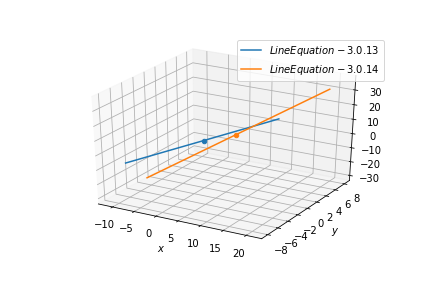
\includegraphics[width=\columnwidth]{./solutions/line_plane/74/codes/figs/Line_interest_2.png}
	\caption{Graph for equations \ref{eq:solutions/line_plane/74/codes14}}
	\label{fig:solutions/line_plane/74/codesline_equation_2}
\end{figure}
\end{enumerate}

    
    
\item 2x+y $\geq$ 6, 3x+4y $\leq$ 12.
    \\
    \solution
    
The given system of inequality can be written in matrix form as
\begin{align}
    \myvec{-1 & -2  \\ -1 & 1 \\ 1 & 1\\ 1 & 0 \\ 0 & 1}\vec{x} \succeq \myvec{-10\\0\\1\\0\\0}
\end{align}
which can be further simplified into 
\begin{align}
    \myvec{-1 & -2 \\ 1 & 0 \\ 0&1}\vec{x} \succeq \myvec{-10\\\frac{-1}{2}\\\frac{-1}{2}}
\end{align}
Let the surplus vector be
\begin{align}
    \vec{u} &= \myvec{u_1\\u_2} \succeq 0
\end{align}
\begin{enumerate}
    \item 
    \begin{align}
        \myvec{-1 & -2 \\ 1 & 0}\vec{x} &\succeq \myvec{-10 \\ \frac{-1}{2}}
        \\
        \implies  \myvec{-1 & -2 \\ 1 & 0}\vec{x} &= \myvec{-10 \\ \frac{-1}{2}} + \vec{u}
    \end{align}
    resulting in 
    \begin{align}
        \vec{x} &= \myvec{-1 & -2 \\ 1 & 0}^{-1}\myvec{-10 \\\frac{-1}{2}} + \myvec{-1 & -2 \\ 1 & 0}^{-1}\vec{u}
        \\
        \implies \vec{x} &= \myvec{\frac{1}{2} \\ \frac{19}{4}} + \myvec{0&1\\ \frac{-1}{2}&\frac{-1}{2}}\vec{u}   \label{ineq/58/eq1}
    \end{align}
    \item 
    \begin{align}
        \myvec{-1& -2 \\ 0 & 1}\vec{x} &\succeq \myvec{-10 \\ \frac{-1}{2}}
        \\
        \implies  \myvec{-1& -2 \\ 0 & 1}\vec{x} &= \myvec{-10 \\ \frac{-1}{2}} + \vec{u}
    \end{align}
    resulting in 
    \begin{align}
        \vec{x} &= \myvec{-1& -2 \\ 0 & 1}^{-1}\myvec{-10 \\ \frac{-1}{2}} + \myvec{-1& -2 \\ 0 & 1}^{-1}\vec{u}
        \\
        \implies \vec{x} &= \myvec{9\\\frac{1}{2}} + \myvec{-1& -2 \\ 0 & 1}\vec{u} \label{ineq/58/eq2}
    \end{align}
\end{enumerate}
Now,solution region which is common to regions of eq. \eqref{ineq/58/eq1} and eq. \eqref{ineq/58/eq2},is given by
\begin{align}
    \boxed{\vec{x} = \myvec{\frac{1}{2}\\\frac{1}{2}}+\myvec{0&1\\\frac{-1}{2}&1}\vec{u}}
\end{align}
%
\begin{figure}[!ht]
\centering
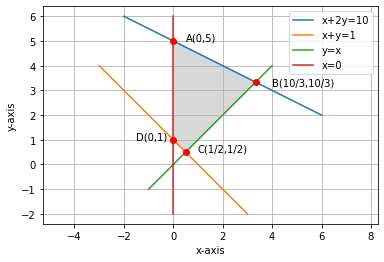
\includegraphics[width=\columnwidth]{solutions/su2021/2/58/Figures/Figure_2.58.png}
\caption{Graphical Solution}
\label{ineq/58/fig:fig1}	
\end{figure}

\begin{figure}[!ht]
\centering
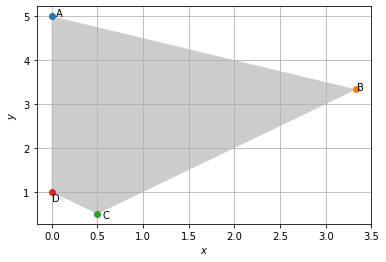
\includegraphics[width=\columnwidth]{solutions/su2021/2/58/Figures/2.58(2).png}
\caption{Magnified Solution region}
\label{ineq/58/fig:fig2}	
\end{figure}


    \item 2x-y $>$ 1, x-2y $<$ -1.
    \\
    \solution
    
%
Let
\begin{align}
\label{eq:1}
\begin{split}
2x-y &> 1,
\\-x+2y &> 1.
\end{split}
\end{align}
\\
Let $u_1 > 0, u_2 > 0$. This may be expressed as
\begin{align}
\vec{u} = \myvec{u_1\\u_2} &> \vec{0}
\end{align}
Now we have,
\begin{align}
\myvec{2&-1 \\ -1&2 }\vec{x} &> \myvec{1 \\ 1}   
\\
\myvec{2&-1 \\ -1&2 }\vec{x}-\vec{u} &= \myvec{1 \\ 1} 
\\
\text{or, } \myvec{2&-1 \\ -1&2 }\vec{x} &= \myvec{1 \\ 1}  + \vec{u}
\end{align}
Resulting in
\begin{align}
\vec{x} &= \myvec{2 & -1 \\ -1 & 2}^{-1}\myvec{1 \\ 1} +\myvec{2 & -1 \\ -1 & 2}^{-1} \vec{u}
\\
\vec{x }&=\myvec{1 \\ 1} +\frac{1}{3}\myvec{2 & 1 \\ 1 & 2}\vec{u}
\end{align} 
Thus , the solution of the system of inequalities can be determined graphically and the desired region is the shaded triangle which is represented in Fig. \ref{fig: Graphical Solution}
\begin{figure}[!ht]
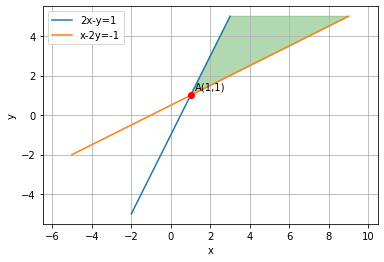
\includegraphics[width=\columnwidth]{solutions/su2021/2/50/Graphical Solution.png}
\caption{Graphical Solution}
\label{fig: Graphical Solution}
\end{figure}



    
\begin{table}[!ht]
\centering
\resizebox{\columnwidth}{!}{\begin{tabular}{|c|c|c|c|} 
\hline
kind of  cake & No.of cakes & Flour& Fat\\
\hline
1st & x & 200g  &  25g \\ 
\hline
2nd& y& 100g&  50g  \\ 
\hline
Total& x+y& 5 kg=5000g&1kg=1000g \\ 
\hline
\end{tabular}}
\caption{Ingredients used in making the cake is flour and fat }
\label{opt/13/tab:table1}
\end{table}
Let the  1st kind  be $x$ and the 2nd kind be $y$  such that 
\begin{align}
x \geq 0 \\
y \geq 0 
\end{align}
According to the question,
\begin{align}
2{x} + {y} \leq 50
\\
{x} + 2{y} \leq 40
\end{align}
$\therefore$ Our problem is
\begin{align}
\max_{\vec{x}} Z &= \myvec{1& 1}\vec{x}\\
s.t. \quad \myvec{2 & 1 \\ 1& 2}\vec{x} &\preceq \myvec{50\\40} 
\end{align}
Lagrangian function is given by
\begin{equation}
\begin{aligned}
&L(\vec{x},\boldsymbol{\lambda}) \\ &= \myvec{1 & 1}\vec{x}+\lcbrak{\sbrak{\myvec{2 & 1}\vec{x}-50}} \\ &+ \sbrak{\myvec{1 & 2}\vec{x}-40}\\ &+ \sbrak{\myvec{-1 & 0}\vec{x}} +\rcbrak{\sbrak{\myvec{0 & -1}\vec{x}}}\boldsymbol{\lambda}
\end{aligned}
\end{equation}
where,
\begin{align}
\boldsymbol{\lambda} &= \myvec{\lambda_1 \\ \lambda_2 \\ \lambda_3 \\ \lambda_4 \\ \lambda_5 \\ \lambda_6}
\end{align}
Now,
\begin{align}
\nabla L(\vec{x},\boldsymbol{\lambda}) &= \myvec{1+ \myvec{2 & 1 & -1 & 0 }\boldsymbol{\lambda}\\ 1+\myvec{1 & 2 & 0 & -1}\boldsymbol{\lambda} \\ \myvec{2 & 1}\vec{x}-50\\ \myvec{1& 2}\vec{x}-40 \\  \myvec{-1 & 0}\vec{x} \\ \myvec{0 & -1}\vec{x}}
\end{align}
$\therefore$ Lagrangian matrix is given by
\begin{align}
\myvec{0 & 0 & 2 & 1& -1 & 0 \\ 0 & 0 & 1 & 2  & 0 & -1 \\ 2 & 1 & 0 & 0 & 0 & 0 \\ 1 & 2 & 0 & 0 & 0 & 0  \\ -1 & 0 & 0 & 0 & 0 & 0  \\ 0 & -1 & 0 & 0 & 0 & 0 }\myvec{\vec{x} \\ \boldsymbol{\lambda} } &= \myvec{-1 \\ -1 \\ 50\\ 4 0\\ 0 \\0 }
\end{align}
Considering $\lambda_1,\lambda_2$ as only active multiplier,
\begin{align}
\myvec{0 & 0 & 2 & 1 \\ 0 & 0 & 1 & 2 \\ 2 & 1 & 0 & 0 \\ 1 & 2 & 0 & 0}\myvec{\vec{x}\\ \boldsymbol{\lambda}} &= \myvec{-1 \\ -1 \\ 5 0\\ 40}
\end{align}
resulting in,
\begin{align}
\myvec{\vec{x} \\ \boldsymbol{\lambda}} &= \myvec{0 & 0 & 2 & 1 \\ 0 & 0 & 1 & 2 \\ 2 & 1 & 0 & 0 \\ 1& 2 & 0 & 0}^{-1}\myvec{-1 \\ -1 \\ 50 \\ 40}
\\
\implies   \myvec{\vec{x} \\ \boldsymbol{\lambda}} &= \myvec{0 & 0 & \frac{2}{3} & \frac{-1}{3} \\ 0 & 0 & \frac{-1}{3} & \frac{2}{3} \\ \frac{2}{3} & \frac{-1}{3} & 0 & 0 \\ \frac{-1}{3} & \frac{2}{3} & 0 & 0}\myvec{-1 \\ -1 \\ 50 \\ 40}
\\
\implies \myvec{\vec{x} \\ \boldsymbol{\lambda}} &= \myvec{20 \\ 10 \\ -0.3 \\ -0.3 }
\end{align}
$\because \boldsymbol{\lambda}=\myvec{-0.3 \\ -0.3} \succ \vec{0} $
\\
$\therefore$ Optimal solution is given by
\begin{align}
    \vec{x} &= \myvec{20\\10} \\
    Z &= \myvec{1& 1}\vec{x} \\
    &= \myvec{1 & 1}\myvec{20 \\ 10} \\
    &= 60
\end{align}
By using cvxpy in python ,
\begin{align}
    \vec{x}=\myvec{20\\10}\\
    Z = 60
\end{align}
Hence No.of cakes \boxed{x=20} 1st kind and  .of cakes \boxed{y=10} 2nd kind should be used to maximum No. of cakes \boxed{Z=60}.  This is
verified in Fig. \ref{opt/13/fig: Graphical Solution}.	
%
\begin{figure}[!ht]
\centering
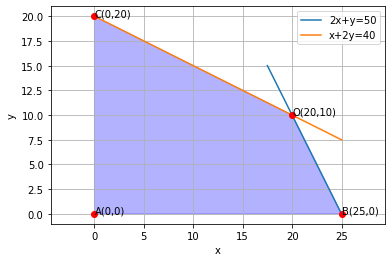
\includegraphics[width=\columnwidth]{solutions/su2021/2/13/Figure9.png}
\caption{Graphical Solution}
\label{opt/13/fig: Graphical Solution}	
\end{figure}

    \item 2x+y $\geq$ 8, x+2y $\geq$ 10.
    \\
    \solution
    
\begin{table}[!ht]
\centering
\resizebox{\columnwidth}{!}{\begin{tabular}{|c|c|c|c|} 
\hline
kind of  cake & No.of cakes & Flour& Fat\\
\hline
1st & x & 200g  &  25g \\ 
\hline
2nd& y& 100g&  50g  \\ 
\hline
Total& x+y& 5 kg=5000g&1kg=1000g \\ 
\hline
\end{tabular}}
\caption{Ingredients used in making the cake is flour and fat }
\label{opt/13/tab:table1}
\end{table}
Let the  1st kind  be $x$ and the 2nd kind be $y$  such that 
\begin{align}
x \geq 0 \\
y \geq 0 
\end{align}
According to the question,
\begin{align}
2{x} + {y} \leq 50
\\
{x} + 2{y} \leq 40
\end{align}
$\therefore$ Our problem is
\begin{align}
\max_{\vec{x}} Z &= \myvec{1& 1}\vec{x}\\
s.t. \quad \myvec{2 & 1 \\ 1& 2}\vec{x} &\preceq \myvec{50\\40} 
\end{align}
Lagrangian function is given by
\begin{equation}
\begin{aligned}
&L(\vec{x},\boldsymbol{\lambda}) \\ &= \myvec{1 & 1}\vec{x}+\lcbrak{\sbrak{\myvec{2 & 1}\vec{x}-50}} \\ &+ \sbrak{\myvec{1 & 2}\vec{x}-40}\\ &+ \sbrak{\myvec{-1 & 0}\vec{x}} +\rcbrak{\sbrak{\myvec{0 & -1}\vec{x}}}\boldsymbol{\lambda}
\end{aligned}
\end{equation}
where,
\begin{align}
\boldsymbol{\lambda} &= \myvec{\lambda_1 \\ \lambda_2 \\ \lambda_3 \\ \lambda_4 \\ \lambda_5 \\ \lambda_6}
\end{align}
Now,
\begin{align}
\nabla L(\vec{x},\boldsymbol{\lambda}) &= \myvec{1+ \myvec{2 & 1 & -1 & 0 }\boldsymbol{\lambda}\\ 1+\myvec{1 & 2 & 0 & -1}\boldsymbol{\lambda} \\ \myvec{2 & 1}\vec{x}-50\\ \myvec{1& 2}\vec{x}-40 \\  \myvec{-1 & 0}\vec{x} \\ \myvec{0 & -1}\vec{x}}
\end{align}
$\therefore$ Lagrangian matrix is given by
\begin{align}
\myvec{0 & 0 & 2 & 1& -1 & 0 \\ 0 & 0 & 1 & 2  & 0 & -1 \\ 2 & 1 & 0 & 0 & 0 & 0 \\ 1 & 2 & 0 & 0 & 0 & 0  \\ -1 & 0 & 0 & 0 & 0 & 0  \\ 0 & -1 & 0 & 0 & 0 & 0 }\myvec{\vec{x} \\ \boldsymbol{\lambda} } &= \myvec{-1 \\ -1 \\ 50\\ 4 0\\ 0 \\0 }
\end{align}
Considering $\lambda_1,\lambda_2$ as only active multiplier,
\begin{align}
\myvec{0 & 0 & 2 & 1 \\ 0 & 0 & 1 & 2 \\ 2 & 1 & 0 & 0 \\ 1 & 2 & 0 & 0}\myvec{\vec{x}\\ \boldsymbol{\lambda}} &= \myvec{-1 \\ -1 \\ 5 0\\ 40}
\end{align}
resulting in,
\begin{align}
\myvec{\vec{x} \\ \boldsymbol{\lambda}} &= \myvec{0 & 0 & 2 & 1 \\ 0 & 0 & 1 & 2 \\ 2 & 1 & 0 & 0 \\ 1& 2 & 0 & 0}^{-1}\myvec{-1 \\ -1 \\ 50 \\ 40}
\\
\implies   \myvec{\vec{x} \\ \boldsymbol{\lambda}} &= \myvec{0 & 0 & \frac{2}{3} & \frac{-1}{3} \\ 0 & 0 & \frac{-1}{3} & \frac{2}{3} \\ \frac{2}{3} & \frac{-1}{3} & 0 & 0 \\ \frac{-1}{3} & \frac{2}{3} & 0 & 0}\myvec{-1 \\ -1 \\ 50 \\ 40}
\\
\implies \myvec{\vec{x} \\ \boldsymbol{\lambda}} &= \myvec{20 \\ 10 \\ -0.3 \\ -0.3 }
\end{align}
$\because \boldsymbol{\lambda}=\myvec{-0.3 \\ -0.3} \succ \vec{0} $
\\
$\therefore$ Optimal solution is given by
\begin{align}
    \vec{x} &= \myvec{20\\10} \\
    Z &= \myvec{1& 1}\vec{x} \\
    &= \myvec{1 & 1}\myvec{20 \\ 10} \\
    &= 60
\end{align}
By using cvxpy in python ,
\begin{align}
    \vec{x}=\myvec{20\\10}\\
    Z = 60
\end{align}
Hence No.of cakes \boxed{x=20} 1st kind and  .of cakes \boxed{y=10} 2nd kind should be used to maximum No. of cakes \boxed{Z=60}.  This is
verified in Fig. \ref{opt/13/fig: Graphical Solution}.	
%
\begin{figure}[!ht]
\centering
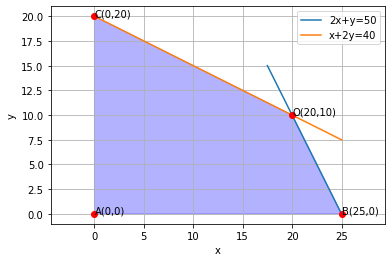
\includegraphics[width=\columnwidth]{solutions/su2021/2/13/Figure9.png}
\caption{Graphical Solution}
\label{opt/13/fig: Graphical Solution}	
\end{figure}

    \item 3x+4y $\leq$ 60, x+3y $\leq$ 30, x $\geq$ 0, y $\geq$ 0.
    \\
    \solution
    
From the given inequalities we have,
\begin{align}
    \myvec{-3&-4 \\ -1&-3 \\ 1&0 \\ 0&1}\vec{x} \succeq \myvec{-60 \\ -30 \\ 0 \\ 0}
\end{align}
Which can be further written as
\begin{align}
   \myvec{-3&-4 \\ -1&-3 }\vec{x} \succeq \myvec{-60 \\ -30} 
\end{align}
Let $u_1 \ge 0, u_2 \ge 0$.  This may be expressed as
\begin{align}
\vec{u} = \myvec{u_1\\u_2}\succeq \vec{0}
\end{align}
Now we have,
\begin{align}
  \myvec{-3&-4 \\ -1&-3 }\vec{x} \succeq \myvec{-60 \\ -30}  + \vec{u} 
\end{align}
\begin{align}
        \vec{x} = \myvec{-3 & -4 \\ -1 & -3}^{-1}\myvec{-60 \\ -30} + \myvec{-3 & -4 \\ -1 & -3}^{-1}\vec{u}
        \\
        \implies \vec{x} = \frac{1}{5}\myvec{60 \\ 30}+\frac{1}{5}\myvec{-3&4 \\ 1&-3}\vec{u}
        \\
        \vec{x}=\myvec{12 \\ 6}+\frac{1}{5}\myvec{-3&4 \\ 1&-3}\vec{u}
    \end{align}
Thus the solution of the system of inequalities can be determined graphically, which is represented in Fig.     \ref{ineq/2/55/Graphical solution}.
%
\begin{figure}[ht]
    \centering
    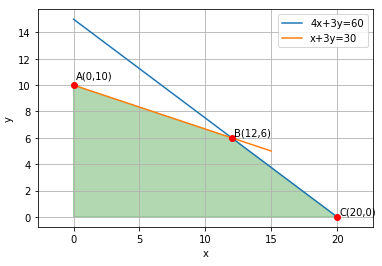
\includegraphics[width=\columnwidth]{solutions/su2021/2/55/Graphical solution region.PNG}
    \caption{Graphical solution}
    \label{ineq/2/55/Graphical solution}
\end{figure}






    \item x-2y $\leq$ 3, 3x+4y $\geq$ 12, x $\geq$ 0, y $\geq$ 1.
    \\
    \solution
    \begin{enumerate}[label=\alph*.]
    \item  Given $\triangle ABC$ with vertices
    \begin{align}
      \vec{A} = \myvec{4 \\ 2}, \vec{B}=\myvec{6 \\ 5},         \vec{C}=\myvec{1 \\ 4}  
    \end{align}
    Given that the median from $\vec{A}$ meets $BC$ at $\vec{D}$, now the coordinate of $\vec{D}$ is given as,
    \begin{align}
        \vec{D} = \frac{\vec{B}+\vec{C}}{2} = \frac{\myvec{6 \\ 5}+\myvec{1 \\ 4}}{2}\\
        \implies \vec{D} = \myvec{\frac{7}{2} \\ \frac{9}{2}}
    \end{align}
    \item  Result :The coordinates of point $\vec{C}$ dividing the line $AB$ in the ratio $m:n$ is given by 
    \begin{align}
      \frac{n\vec{A}+m\vec{B}}{m+n}  \label{vectors/2/eq:1}
    \end{align}
    Given that the point $\vec{P}$ divides $AD$ in the ratio $2:1$, now to find $\vec{P}$ we use \eqref{vectors/2/eq:1},
    \begin{align}
        \vec{P}=\frac{1\myvec{4\\2}+2\myvec{\frac{7}{2}\\ \frac{9}{2}}}{3}=\myvec{\frac{11}{3} \\ \frac{11}{3}}
    \end{align}
    \item Given that the point $\vec{Q}$ on the median $BE$ divides it in the ratio $2:1$, first we find $\vec{E}$,
    \begin{align}
        \vec{E} =\frac{\vec{A}+\vec{C}}{2} = \frac{\myvec{4 \\ 2}+\myvec{1 \\ 4}}{2}\\
        \implies \vec{E} = \myvec{\frac{5}{2} \\ 3}.
    \end{align}
    Now we find $\vec{Q}$ using \eqref{vectors/2/eq:1}
    \begin{align}
       \vec{Q}=\frac{1\myvec{6\\5}+2\myvec{\frac{5}{2}\\3}}{3}=\myvec{\frac{11}{3} \\ \frac{11}{3}} 
    \end{align}
    Similarly,Given that the point $\vec{R}$ on the median $CF$ divides it in the ratio $2:1$, first we find $\vec{F}$,
    \begin{align}
        \vec{F} =\frac{\vec{A}+\vec{B}}{2} = \frac{\myvec{4 \\ 2}+\myvec{6 \\ 5}}{2}\\
        \implies \vec{F} = \myvec{5 \\ \frac{7}{2}}.
    \end{align}
    Now we find $\vec{R}$ using \eqref{vectors/2/eq:1}
    \begin{align}
       \vec{R}=\frac{1\myvec{1\\4}+2\myvec{5 \\ \frac{7}{2}}}{3}=\myvec{\frac{11}{3} \\ \frac{11}{3}} 
    \end{align}
    \end{enumerate}
    The plot of the $\triangle ABC$ is given in Fig.     \ref{vectors/2/fig:triangle ABC}.
    %
    \begin{figure}[ht]
        \centering
        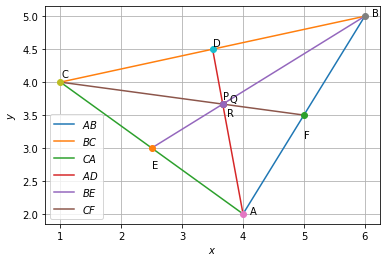
\includegraphics[width=\columnwidth]{solutions/su2021/2/2/TriangleABC.PNG}
        \caption{Plot of $\triangle ABC$}
        \label{vectors/2/fig:triangle ABC}
    \end{figure}
    \item 4x+3y $\leq$ 60, y $\geq$ 2x, x $\geq$ 3, x,y $\geq$ 0.
    \\
    \solution
    

The given system of inequality can be written in matrix form as
\begin{align}
    \myvec{-4 & -3 \\ -2 & 1 \\ 1 & 0 \\ 1 & 0 \\ 0 & 1}\vec{x} \succeq \myvec{-60\\0\\3\\0\\0}
\end{align}
which can be further simplified into 
\begin{align}
    \myvec{-4 & -3 \\ 1 & 0 \\ 0 & 1}\vec{x} \succeq \myvec{-60\\3\\6}
\end{align}

Let the surplus vector be
\begin{align}
    \vec{u} &= \myvec{u_1\\u_2} \succeq 0
\end{align}

\begin{enumerate}
    \item 
    \begin{align}
        \myvec{-4 & -3 \\ 1 & 0}\vec{x} &\succeq \myvec{-60 \\ 3}
        \\
        \implies  \myvec{-4 & -3 \\ 1 & 0}\vec{x} &= \myvec{-60 \\ 3} + \vec{u}
    \end{align}
    resulting in 
    \begin{align}
        \vec{x} &= \myvec{-4 & -3 \\1 & 0}^{-1}\myvec{-60 \\ 3} + \myvec{-4 & -3 \\1 & 0}^{-1}\vec{u}
        \\
        \implies \vec{x} &= \myvec{3 \\16} + \myvec{0 & 1\\ \frac{-1}{3} & \frac{-4}{3}}\vec{u}   \label{ineq/2/57eq1}
    \end{align}

    \item 
    \begin{align}
        \myvec{-4 & -3 \\ 0 & 1}\vec{x} &\succeq \myvec{-60 \\ 6}
        \\
        \implies  \myvec{-4 & -3 \\ 0 & 1}\vec{x} &= \myvec{-60 \\ 6} + \vec{u}
    \end{align}
    resulting in 
    \begin{align}
        \vec{x} &= \myvec{-4 & -3 \\0 & 1}^{-1}\myvec{-60 \\ 6} + \myvec{-4 & -3 \\0 & 1}^{-1}\vec{u}
        \\
        \implies \vec{x} &= \myvec{\frac{21}{2} \\6} + \myvec{\frac{-1}{4} & \frac{-3}{4}\\ 0 & 1}\vec{u} \label{ineq/2/57eq2}
    \end{align}
\end{enumerate}

Now,solution region which is common to regions of eq. \eqref{ineq/2/57eq1} and eq. \eqref{ineq/2/57eq2},is given by

\begin{align}
    \boxed{\vec{x} = \myvec{3 \\ 6}+\myvec{0 & 1\\\frac{1}{12} & \frac{-13}{12}}\vec{u}}
\end{align}


\begin{figure}[!ht]
\centering
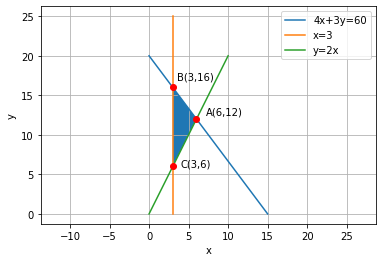
\includegraphics[width=\columnwidth]{solutions/su2021/2/57/Figures/Figure11_1.png}
\caption{Solution Region}
\label{ineq/2/57fig:fig1}	
\end{figure}

% \numberwithin{figure}{section}
% \begin{figure}[!ht]
% \centering
% 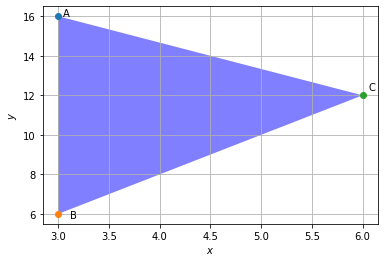
\includegraphics[width=\columnwidth]{Figure11_2}
% \caption{Magnified Solution Region}
% \label{ineq/2/57fig:fig2}	
% \end{figure}




%\end{document}

